\documentclass[a4paper]{article}

% PACKAGES
\usepackage[bahasa]{babel}
\usepackage[utf8]{inputenc}
\usepackage{amsmath, amssymb}
\usepackage{graphicx}
\usepackage{tikz,pgfplots}
\pgfplotsset{compat=1.18}
\usetikzlibrary{positioning, arrows.meta}
\usepackage{booktabs}
\usepackage{caption}
\usepackage[
    backend=biber,
    style=ieee,
    sorting=none
]{biblatex}
\usepackage{hyperref}
\hypersetup{
    colorlinks=true,
    linkcolor=blue,
    citecolor=red,
    urlcolor=cyan,
}
\usepackage{geometry}
\usepackage{abstract}
\setlength{\absleftindent}{0pt}
\setlength{\absrightindent}{0pt}
% Ubah judul lingkungan abstract ke Bahasa Indonesia
\renewcommand{\abstractname}{Abstrak}

% BIBLIOGRAPHY
\addbibresource{references.bib}

% KEYWORDS ENVIRONMENT
\newcommand{\keywords}[1]{%
  \begin{center}
  \textbf{\textit{Kata Kunci---}}#1
  \end{center}
}

% DOCUMENT INFO
\title{\textbf{Aplikasi Deret Fourier: Transformasi Kosinus Diskrit (DCT) dalam Kompresi Citra Digital JPEG}}
\author{Teosofi Hidayah Agung\\5002221132}
\date{\today}

\begin{document}

\maketitle

\begin{abstract}
  Makalah ini menyajikan telaah mendalam mengenai aplikasi Deret Fourier, khususnya Transformasi Kosinus Diskrit (DCT), sebagai landasan matematis dari standar kompresi citra JPEG. Pembahasan dimulai dari evolusi konsep analisis frekuensi, mulai dari Deret Fourier untuk sinyal periodik, Transformasi Fourier untuk sinyal non-periodik, hingga adaptasi digital melalui Transformasi Fourier Diskrit (DFT). Analisis difokuskan pada keunggulan fundamental DCT, yaitu properti pemadatan energi (\textit{energy compaction}) yang superior, yang memungkinkannya mengkonsentrasikan informasi visual penting ke dalam sejumlah kecil koefisien. Selanjutnya, makalah ini membedah anatomi lengkap alur kerja kompresi JPEG, mulai dari pra-pemrosesan, kuantisasi, hingga pengkodean entropi. Analisis kinerja juga disajikan, menguraikan hubungan antara tingkat kompresi dan munculnya artefak visual seperti \textit{blocking} dan \textit{ringing}. Terakhir, JPEG ditempatkan dalam konteks evolusi teknologi dengan membandingkannya dengan standar yang lebih modern seperti JPEG 2000, WebP, dan AVIF untuk memberikan gambaran masa depan kompresi citra.
\end{abstract}

\keywords{Deret Fourier, Transformasi Kosinus Diskrit, JPEG, Kompresi Citra, Artefak Kompresi.}

\section{Pendahuluan}
Analisis Fourier adalah fondasi yang memungkinkan representasi sinyal dan citra dalam domain frekuensi; konsep ini menjelaskan mengapa transformasi seperti DCT mampu memusatkan energi dan mengurangi redundansi visual secara efektif. Sebagai pengantar singkat, pemahaman mengenai dekomposisi sinyal ke komponen frekuensi membantu menjelaskan perilaku \textit{transform-domain compression}.

Standar JPEG, yang berlandaskan pada DCT, telah lama menjadi solusi praktis untuk kompresi citra \textit{lossy} karena kombinasi efisiensi komputasi, pemadatan energi yang baik, dan dukungan perangkat keras/ekosistem yang luas.

Studi terhadap JPEG relevan secara praktis karena desainnya merepresentasikan trade-off nyata antara efisiensi dan kualitas visual: penggunaan blok $8\times 8$ dan kuantisasi memberikan pengurangan bit-rate yang signifikan namun juga menimbulkan artefak seperti \textit{blocking} dan \textit{ringing} pada tingkat kompresi tinggi. Dengan menganalisis bagaimana DCT memusatkan energi, bagaimana kuantisasi memengaruhi distribusi koefisien frekuensi, serta bagaimana pilihan parameter (mis. ukuran blok, matriks kuantisasi, dan strategi kuantisasi) berdampak pada persepsi visual, kita memperoleh landasan untuk menilai dan menyesuaikan algoritme kompresi pada situasi nyata — dari penyimpanan hingga transmisi dan pemrosesan citra. Oleh karena itu, memahami aspek-aspek praktis ini membantu jembatani teori transformasi frekuensi dengan keputusan implementasi yang menentukan kualitas akhir citra.

\section{Formulasi Deret Fourier dan Transformasi Fourier}
\subsection{Esensi Deret Fourier}
Setiap fungsi periodik dapat diuraikan sebagai deret tak hingga dari jumlahan fungsi sinus dan kosinus dengan berbagai frekuensi dan amplitudo \cite{bracewell1999fourier}. Deret Fourier untuk fungsi periodik $f(t)$ dengan periode $2L$ dinyatakan sebagai:
\begin{equation} \label{eq:fourier_series}
  f(t) = \frac{a_0}{2} + \sum_{n=1}^{\infty} \left( a_n \cos\left(\frac{n\pi t}{L}\right) + b_n \sin\left(\frac{n\pi t}{L}\right) \right)
\end{equation}
di mana koefisien $a_0$, $a_n$, dan $b_n$ dihitung menggunakan integral berikut \cite{oppenheim1996signals}:
\begin{gather}
  a_0 = \frac{1}{L} \int_{-L}^{L} f(t) \,dt \label{eq:a0} \\
  a_n = \frac{1}{L} \int_{-L}^{L} f(t) \cos\left(\frac{n\pi t}{L}\right) \,dt \label{eq:an} \\
  b_n = \frac{1}{L} \int_{-L}^{L} f(t) \sin\left(\frac{n\pi t}{L}\right) \,dt \label{eq:bn}
\end{gather}
Dekomposisi ini adalah transformasi dari domain waktu ke domain frekuensi. Sifat simetri fungsi asli berdampak langsung pada koefisiennya; fungsi genap hanya menghasilkan suku kosinus, sedangkan fungsi ganjil hanya menghasilkan suku sinus \cite{bracewell1999fourier}.

\subsection{Transformasi Fourier untuk Sinyal Non-Periodik}
Untuk sinyal non-periodik, konsep Deret Fourier diperluas dengan memperlakukan sinyal sebagai periodik dengan periode mendekati tak hingga ($T \to \infty$) \cite{bracewell1999fourier}. Dalam limit ini, spektrum frekuensi menjadi kontinu dan jumlahan berubah menjadi integral, melahirkan pasangan Transformasi Fourier:
\begin{gather}
  F(\omega) = \int_{-\infty}^{\infty} f(t) e^{-j\omega t} \,dt \label{eq:ft_forward} \\
  f(t) = \frac{1}{2\pi} \int_{-\infty}^{\infty} F(\omega) e^{j\omega t} \,d\omega \label{eq:ft_inverse}
\end{gather}
Untuk citra 2D, digunakan Transformasi Fourier 2D kontinu. Namun, bentuk ini tidak dapat dihitung secara langsung oleh komputer karena melibatkan operasi integral pada fungsi kontinu \cite{oppenheim1996signals}.

\subsection{Transformasi Fourier Diskrit (DFT)}
Untuk aplikasi digital, Transformasi Fourier Diskrit (DFT) dikembangkan. DFT diterapkan pada sinyal yang telah diambil sampelnya (diskrit) dan menghasilkan spektrum frekuensi yang juga diskrit. Untuk sekuens data 1D $f[n]$ dengan $N$ sampel, DFT didefinisikan sebagai \cite{oppenheim1996signals}:
\begin{equation} \label{eq:dft_1d}
  F[k] = \sum_{n=0}^{N-1} f[n] e^{-j\frac{2\pi kn}{N}}, \quad k = 0, \dots, N-1
\end{equation}
Meskipun dapat diimplementasikan secara komputasi, DFT memiliki dua kelemahan fundamental untuk kompresi citra:
\begin{itemize}
  \item Menghasilkan output bilangan kompleks, yang tidak efisien untuk disimpan.
  \item Asumsi periodisitas implisit menciptakan diskontinuitas artifisial pada batas blok citra, menghasilkan banyak koefisien frekuensi tinggi yang tidak perlu \cite{ucsd_dct_notes}.
\end{itemize}

\subsection{Hubungan DFT, DCT, dan DST}

Dengan memisahkan komponen real dan imajiner dari \eqref{eq:dft_1d}, diperoleh:
\begin{equation}
  F[k] = \sum_{n=0}^{N-1} x[n] \left[ \cos\left( \frac{2\pi kn}{N} \right) - j \sin\left( \frac{2\pi kn}{N} \right) \right].
\end{equation}

Jika sinyal diperluas secara \textit{even symmetric}, maka komponen sinus akan hilang dan tersisa hanya kosinus. Hasilnya adalah:
\begin{equation}
  F_c[k] = \sum_{n=0}^{N-1} x[n] \cos \left[ \frac{\pi}{N} \left( n + \frac{1}{2} \right) k \right],
  \quad k = 0, 1, \ldots, N-1
\end{equation}
yang dikenal sebagai \textbf{DCT-II}.

Jika sinyal diperluas secara \textit{odd symmetric}, maka komponen kosinus akan hilang dan tersisa hanya sinus:
\begin{equation}
  F_s[k] = \sum_{n=0}^{N-1} x[n] \sin \left[ \frac{\pi}{N+1} (n + 1)(k + 1) \right],
  \quad k = 0, 1, \ldots, N-1.
\end{equation}

Dengan demikian, baik DCT maupun DST dapat dianggap sebagai versi \textit{real-valued} dari DFT yang didesain untuk memenuhi kondisi batas tertentu.


\section{Transformasi Kosinus Diskrit (DCT)}
DCT muncul sebagai solusi yang dirancang untuk mengatasi kelemahan DFT. DCT tidak hanya menghasilkan koefisien riil, tetapi juga memiliki properti "pemadatan energi" yang jauh lebih unggul, yang menjadi kunci keberhasilan standar kompresi JPEG \cite{wallace1991jpeg}.

\subsection{Definisi Matematis}
DCT pertama kali diperkenalkan oleh Ahmed, Natarajan, dan Rao pada tahun 1974 \cite{ahmed1974dct}. Berbeda dengan DFT, DCT hanya menggunakan basis fungsi kosinus, sehingga input riil (nilai piksel) akan selalu menghasilkan output riil \cite{ucsd_dct_notes}. Varian yang paling umum digunakan dalam kompresi citra adalah DCT-II, yang untuk sekuens 1D $f[n]$ didefinisikan sebagai:
\begin{equation} \label{eq:dct_1d}
  F[k] = c[k] \sum_{n=0}^{N-1} f[n] \cos\left(\frac{(2n+1)k\pi}{2N}\right)
\end{equation}
di mana $c[k]$ adalah faktor normalisasi. Untuk aplikasi citra 2D pada blok $N \times N$, digunakan formula 2D-DCT yang dapat dipisahkan (\textit{separable}). Secara konseptual, menerapkan DCT-II pada $N$ titik setara dengan mengambil DFT dari sekuens yang telah diperpanjang secara simetris menjadi $2N$ titik, yang secara efektif menghilangkan diskontinuitas pada batas blok \cite{ucsd_dct_notes}.

\subsection{DCT pada 2-Dimensi}
DCT pada 2-dimensi diterapkan pada blok citra $N \times N$ dengan cara yang dapat dipisahkan. Ini berarti bahwa DCT dapat diterapkan secara terpisah pada setiap baris dan kolom blok citra. Secara matematis, DCT 2D untuk blok citra $f[x,y]$ didefinisikan sebagai:
\begin{equation} \label{eq:dct_2d}
  F_{[u,v]}(x,y) = \frac{1}{4} \alpha[u] \alpha[v] \sum_{x=0}^{N-1} \sum_{y=0}^{N-1} f(x,y) \cos\left(\frac{(2x+1)u\pi}{2N}\right) \cos\left(\frac{(2y+1)v\pi}{2N}\right)
\end{equation}
di mana $\alpha[u]$ dan $\alpha[v]$ adalah faktor normalisasi yang didefinisikan sebagai:
\begin{equation}
  \alpha[k] =
  \begin{cases}
    \frac{1}{\sqrt{N}},  & k = 0,   \\[4pt]
    \frac{1}{\sqrt{2N}}, & k \ge 1.
  \end{cases}
\end{equation}

\section{Anatomi Standar Kompresi JPEG}
Standar kompresi JPEG adalah proses multi-tahap yang dirancang untuk mengurangi ukuran file citra secara signifikan, di mana setiap langkah bekerja secara sinergis \cite{wallace1991jpeg}.

\subsection{Pra-pemrosesan}
Langkah pertama untuk citra berwarna adalah transformasi ruang warna dari RGB ke YCbCr, yang memisahkan komponen kecerahan (Y) dari komponen warna (Cb, Cr). Karena mata manusia kurang sensitif terhadap perubahan warna, resolusi spasial komponen Cb dan Cr dikurangi melalui teknik \textit{chroma subsampling}, yang merupakan langkah kompresi pertama yang sangat efisien \cite{wallace1991jpeg}.

Transformasi dari ruang warna RGB ke ruang Y'CbCr pada standar terbaru, yaitu \textit{ITU-R BT.2020},
didefinisikan dengan mempertimbangkan sifat non-linear dari sistem tampilan modern \cite{itu2020}.
Pada standar ini, komponen warna yang digunakan adalah $R'$, $G'$, dan $B'$,
yakni hasil dari penerapan fungsi \textit{gamma correction} terhadap nilai RGB linear.
Fungsi non-linear tersebut diberikan oleh:
\begin{equation}
  f(x) =
  \begin{cases}
    4.5x,                  & x < 0.018,   \\[4pt]
    1.099x^{0.45} - 0.099, & x \ge 0.018,
  \end{cases}
\end{equation}
sehingga diperoleh $R' = f(R)$, $G' = f(G)$, dan $B' = f(B)$.

Selanjutnya, komponen luminansi ($Y'$) serta dua komponen krominansi ($Cb$, $Cr$) dihitung menggunakan kombinasi linier dari $R'$, $G'$, dan $B'$ sebagai berikut:
\begin{equation}
  \begin{bmatrix}
    Y' \\[4pt]
    Cb \\[4pt]
    Cr
  \end{bmatrix}
  =
  \begin{bmatrix}
    0.2627   & 0.6780   & 0.0593   \\[4pt]
    -0.13963 & -0.36037 & 0.50000  \\[4pt]
    0.50000  & -0.45979 & -0.04021
  \end{bmatrix}
  \begin{bmatrix}
    R' \\[4pt]
    G' \\[4pt]
    B'
  \end{bmatrix}.
\end{equation}

Koefisien pada matriks di atas diturunkan dari nilai konstanta primaries standar BT.2020, yaitu
$K_R = 0.2627$, $K_B = 0.0593$, dan $K_G = 1 - K_R - K_B = 0.6780$.
Pendekatan ini memungkinkan representasi luminansi ($Y'$) yang konsisten dengan persepsi visual manusia,
serta menghasilkan rentang warna (\textit{color gamut}) yang lebih luas pada sistem tampilan berdefinisi tinggi.
\begin{figure}[h!]
  \centering
  \begin{tikzpicture}[
      node distance=0.5cm and 4cm,
      every node/.style={align=center, font=\small},
      box/.style={rectangle, draw, rounded corners, thick, fill=gray!10},
      arrow/.style={->, thick, >=stealth}
    ]

    % === Gambar Asli ===
    \node[box] (rgb) {\includegraphics[width=7cm]{img/100.jpg} \\ \textbf{Gambar RGB Asli}};

    % === Komponen Hasil ===
    \node[box, below left=of rgb.south east, xshift=-3.2cm, yshift=-0.3cm] (Y) {\includegraphics[width=3cm]{img/Y_100.jpg} \\ \textbf{Komponen Y}};
    \node[box, below=of rgb.south, yshift=-0.3cm] (Cb) {\includegraphics[width=3cm]{img/Cb_100.jpg} \\ \textbf{Komponen Cb}};
    \node[box, below right=of rgb.south west, xshift=3.2cm, yshift=-0.3cm] (Cr) {\includegraphics[width=3cm]{img/Cr_100.jpg} \\ \textbf{Komponen Cr}};

    % === Panah Hubungan ===
    \draw[arrow] (rgb.south) -- ++(0,-0.2) -| (Y.north);
    \draw[arrow] (rgb.south) -- (Cb.north);
    \draw[arrow] (rgb.south) -- ++(0,-0.2) -| (Cr.north);

  \end{tikzpicture}
  \caption{Gambar RGB dipecah menjadi tiga komponen: Y, Cb, dan Cr.}
  \label{fig:rgb_to_ycbcr}
\end{figure}

\subsection{Partisi Blok}
Setiap kanal (Y, Cb, Cr) dibagi menjadi blok-blok $8 \times 8$ piksel. Nilai piksel dalam setiap blok digeser levelnya menjadi rentang [-128, 127] dari yang semula [0, 255], kemudian 2D-DCT diterapkan pada setiap blok, mengubah 64 nilai piksel spasial menjadi 64 koefisien frekuensi.

\begin{figure}[h!]
  \centering
  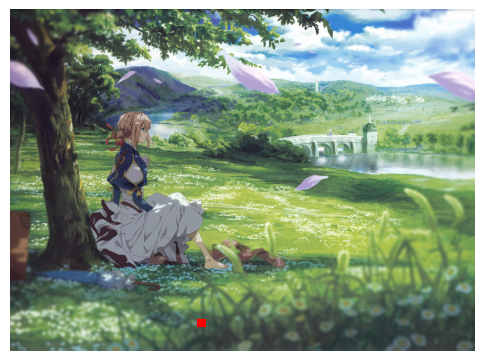
\includegraphics[width=0.3\textwidth]{img/partition1.png}\qquad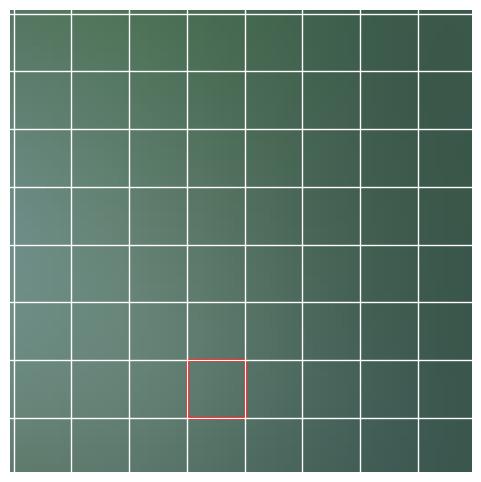
\includegraphics[width=0.2\textwidth]{img/partition2.png}\qquad
\includegraphics[width=0.2\textwidth]{img/partition3.png}
  \caption{Partisi blok $64 \times 64$ dilanjutkan dengan $8\times 8$ pada citra luminansi.}
  \label{fig:block_partition}
\end{figure}

Selanjutnya, blok-blok ini dapat diproses dalam ukuran yang lebih besar, seperti $16 \times 16$ atau $32 \times 32$, untuk mengurangi overhead pemrosesan. Namun, ukuran blok yang lebih besar cenderung menghasilkan artefak visual yang lebih jelas, terutama pada tingkat kompresi tinggi. Oleh karena itu, standar JPEG memilih ukuran blok $8 \times 8$ sebagai kompromi optimal antara efisiensi kompresi dan kualitas visual \cite{wallace1991jpeg}. Sebagai tambahan informasi, pada gambar \ref{fig:block_partition} bisa diperoleh matriks $8 \times 8$ dari blok yang dipilih sebagai berikut:
\[
  \begin{bmatrix}
    114 & 113 & 111 & 110 & 109 & 108 & 107 & 106 \\
    113 & 112 & 111 & 110 & 109 & 108 & 107 & 105 \\
    113 & 112 & 111 & 110 & 109 & 108 & 106 & 105 \\
    113 & 112 & 111 & 110 & 108 & 107 & 106 & 105 \\
    112 & 111 & 110 & 109 & 108 & 107 & 106 & 105 \\
    112 & 111 & 110 & 109 & 108 & 107 & 106 & 104 \\
    111 & 110 & 109 & 108 & 107 & 106 & 105 & 104 \\
    111 & 110 & 109 & 108 & 107 & 106 & 105 & 104
  \end{bmatrix}
\]

\subsection{Aplikasi DCT}
Pertama jika kita tinjau salah satu baris piksel dari citra \textit{grayscale} (Y), misalnya baris ke-100 dari citra $6660 \times 4898$ piksel Gambar \ref{fig:rgb_to_ycbcr}.
\begin{figure}[h!]
  \centering
  \begin{tikzpicture}[
      node distance=1.5cm and 0.5cm,
      every node/.style={align=center, font=\small},
      box/.style={rectangle, draw, rounded corners, thick, fill=gray!10},
      arrow/.style={->, thick, >=stealth}
    ]

    % === Gambar Asli ===
    \node[] (rgb) {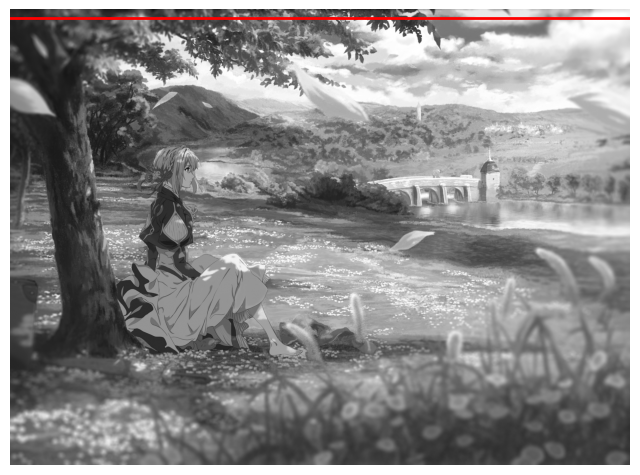
\includegraphics[width=6cm]{img/Y100.png}};

    % === Komponen Hasil ===
    \node[right=of rgb.east, yshift=2cm] (strip) {
\includegraphics[width=7.2cm]{img/strip.png}};
    \node[right=of rgb.east, yshift=0cm] (graph) {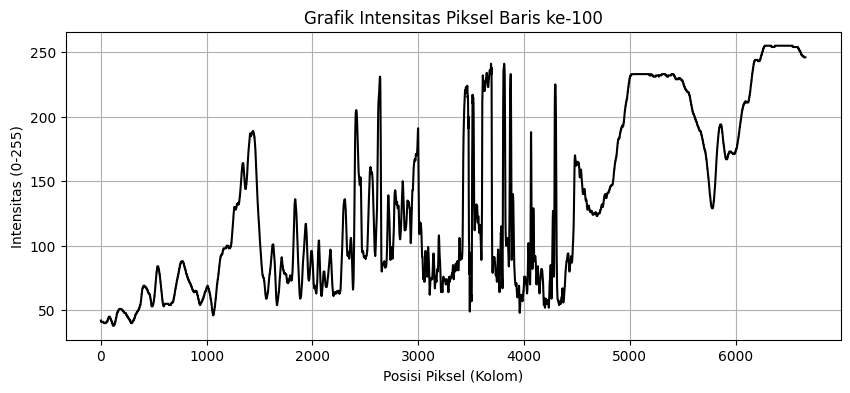
\includegraphics[width=7.2cm]{img/graph.png}};

    % === Panah Hubungan ===
    \draw[arrow] (rgb.32) -- (strip.west);
    \draw[arrow] (rgb.32) -- (graph.west);

  \end{tikzpicture}
  \caption{Visualisasi baris piksel sebagai strip horizontal dan grafik intensitasnya.}
  \label{fig:line_pixel_visualization}
\end{figure}
Perhatikan pada Gambar \ref{fig:line_pixel_visualization} bahwa perbaris piksel dari komponen Y (\textit{luminance}) dapat kita pandang sebagai grafik intensitas piksel terhadap posisi horizontalnya. Grafik ini dapat kita anggap sebagai sinyal 1D yang diskrit dan terhingga, sehingga kita dapat menerapkan DCT 1D (\ref{eq:dct_1d}) untuk menganalisis komponen frekuensinya.

Pada kasus kompresi JPEG, DCT 2D diterapkan pada total $64$ blok. Dengan menggunakan pengetahuan tentang Aljabar Linear, kita dapat mengekspresikan blok $8 \times 8$ sebagai kombinasi linier dari basis DCT 2D. Basis ini diambil dari persamaan (\ref{eq:dct_2d}) dengan memasukkan nilai $f(x,y)=1$. Sehingga disajikan dalam bentuk fungsi dua variabel $B_{[u,v]}(x,y)$ sebagai berikut:
\begin{equation}
  B_{[u,v]}(x,y) = \frac{1}{4} \alpha[u] \alpha[v] \cos\left(\frac{(2x+1)u\pi}{16}\right) \cos\left(\frac{(2y+1)v\pi}{16}\right)
\end{equation}
dengan $u,v,x,y = 0,1,\ldots,7$ dan
\begin{align}
  \alpha[k] =
  \begin{cases}
    \frac{1}{\sqrt{8}}, & k = 0, \\
    \frac{1}{2},        & k > 0.
  \end{cases}
\end{align}

\begin{figure}[h]
  \centering
  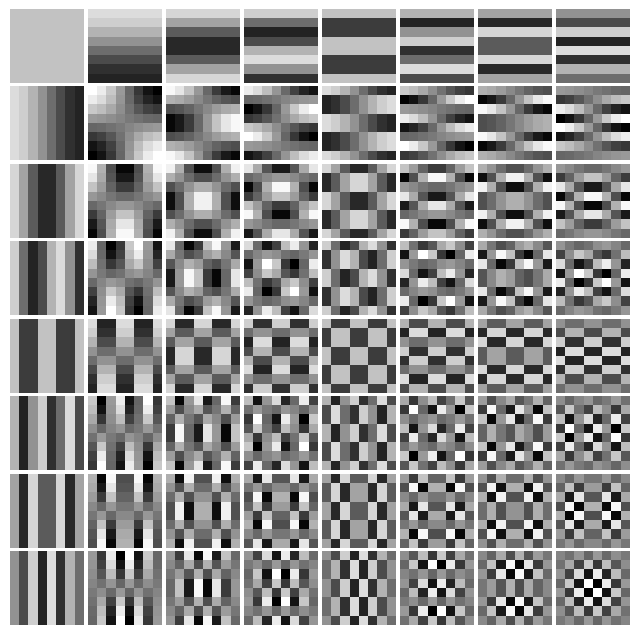
\includegraphics[width=0.4\textwidth]{img/DCTbasis.png}
  \begin{tikzpicture}[scale=0.7, every node/.style={font=\scriptsize, align=center}]
    % Ukuran kotak
    \def\s{1.0}

    % grid 8x8
    \foreach \u in {0,...,7}{
        \foreach \v in {0,...,7}{
            \pgfmathsetmacro{\x}{\v*\s}
            \pgfmathsetmacro{\y}{-1*\u*\s}
            % gambar kotak
            \draw[thick] (\x,\y) rectangle ++(\s,-\s);
            % label di tengah
            \node at (\x+0.5*\s,\y-0.5*\s)
            {$B_{{[\u,\v]}}$};
          }
      }
  \end{tikzpicture}
  \caption{Basis DCT 2D untuk blok $8 \times 8$.}
  \label{fig:dct_basis}
\end{figure}

Gambar \ref{fig:dct_basis} menampilkan 64 basis DCT 2D yang digunakan untuk merepresentasikan blok $8 \times 8$. Basis ini diurutkan berdasarkan frekuensi spasialnya, dari frekuensi rendah di kiri atas hingga frekuensi tinggi di kanan bawah. Setiap basis dapat dianggap sebagai pola gelombang kosinus dengan frekuensi tertentu dalam arah horizontal dan vertikal.

\subsection{Kuantisasi: Kompresi \textit{Lossy}}
Kuantisasi adalah satu-satunya tahap di mana informasi hilang secara permanen. Prosesnya melibatkan pembagian setiap koefisien DCT dengan nilai dari matriks kuantisasi, lalu hasilnya dibulatkan ke bilangan bulat terdekat.
\begin{equation} \label{eq:quantization}
  F_Q[u, v] = \text{round}\left(\frac{F[u, v]}{Q[u, v]}\right)
\end{equation}
Matriks kuantisasi $Q[u,v]$ dirancang berdasarkan sensitivitas visual manusia, dengan nilai kecil untuk frekuensi rendah dan besar untuk frekuensi tinggi. Ini berarti koefisien frekuensi tinggi yang kurang penting secara perseptual akan dikurangi secara drastis, sering kali menjadi nol \cite{wallace1991jpeg}.

\subsection{Serialisasi dan Pengkodean Entropi}
Setelah kuantisasi, matriks $8 \times 8$ yang "jarang" diubah menjadi vektor 1D menggunakan pemindaian zig-zag. Pola ini mengelompokkan koefisien non-nol di awal vektor dan menciptakan barisan panjang nilai nol di akhir. Vektor ini kemudian dikodekan secara \textit{lossless} menggunakan DPCM untuk koefisien DC dan RLE untuk koefisien AC, diikuti oleh pengkodean Huffman untuk merepresentasikan data akhir seefisien mungkin \cite{wallace1991jpeg}.

\subsection{Proses Dekompresi}
Untuk merekonstruksi citra, seluruh proses dilakukan secara terbalik: Dekode Entropi, De-serialisasi, De-kuantisasi, dan Transformasi Kosinus Diskrit Terbalik (IDCT). Pada IDCT, koefisien frekuensi dikonversi kembali ke domain spasial menggunakan sifat dari keorthonormalan basis DCT \cite{wallace1991jpeg}.
\begin{equation}
  f(x,y) = \frac{1}{4} \sum_{u=0}^{7} \sum_{v=0}^{7} \alpha[u] \alpha[v] F_{[u,v]}(x,y) \cos\left(\frac{(2x+1)u\pi}{16}\right) \cos\left(\frac{(2y+1)v\pi}{16}\right)
\end{equation}

\section{Analisis Kinerja dan Artefak Visual}
Efektivitas JPEG diukur dari rasio kompresi dan kualitas visual, yang merupakan sebuah pertukaran (\textit{trade-off}).

\begin{figure}[h]
  \centering
  
\includegraphics[width=0.3\textwidth]{img/nijika1.jpg}\qquad
\includegraphics[width=0.3\textwidth]{img/nijika2.jpg}\qquad
\includegraphics[width=0.3\textwidth]{img/nijika3.jpg}
  \caption{Artefak visual pada citra JPEG berbanding lurus dengan tingkat kompresi}
\end{figure}

\subsection{Keunggulan dan Kelemahan}
Keunggulan utama JPEG adalah rasio kompresi yang sangat tinggi pada citra fotografi dengan degradasi perseptual minimal pada kualitas tinggi \cite{wallace1991jpeg}. Namun, sifatnya yang \textit{lossy} berarti kualitas citra menurun setiap kali disimpan ulang. Pada kompresi tinggi, artefak visual menjadi jelas terlihat.

\subsection{Artefak Visual Kompresi}
\begin{itemize}
  \item \textbf{Artefak Pemblokiran (\textit{Blocking Artifacts}):} Muncul sebagai pola kisi-kisi $8\times 8$, terutama di area gradasi halus. Ini disebabkan oleh pemrosesan independen pada setiap blok dan kuantisasi kasar yang menciptakan batas artifisial antar blok \cite{singh2012blocking, chou1998smoothing}.
  \item \textbf{\textit{Ringing} dan \textit{Blurring}:} \textit{Blurring} terjadi ketika koefisien frekuensi tinggi (detail halus) dihilangkan. \textit{Ringing} muncul sebagai "gema" di sekitar tepi kontras tinggi, sebuah manifestasi dari Fenomena Gibbs akibat pembuangan komponen frekuensi tinggi yang diperlukan untuk merekonstruksi tepi yang tajam \cite{gottlieb1996gibbs, marziliano2004perceptual}.
\end{itemize}

\begin{table}[h!]
  \centering
  \caption{Perbandingan Kualitas vs. Tingkat Kompresi JPEG}
  \label{tab:kualitas_jpeg}
  \begin{tabular*}{\columnwidth}{@{\extracolsep{\fill}}lll@{}}
    \toprule
    \textbf{Kualitas (\%)} & \textbf{Rasio Kompresi} & \textbf{Deskripsi Artefak Visual}                     \\ \midrule
    95-100                 & 2:1 - 5:1               & Artefak hampir tidak terlihat.                        \\
    85-94                  & 5:1 - 15:1              & Kualitas sangat baik untuk sebagian besar penggunaan. \\
    75-84                  & 15:1 - 25:1             & Keseimbangan baik, artefak mulai terlihat.            \\
    50-74                  & 25:1 - 40:1             & Artefak jelas, detail mulai hilang.                   \\
    <50                    & > 40:1                  & Degradasi citra sangat parah.                         \\ \bottomrule
  \end{tabular*}
\end{table}

\section{Contoh Penerapan dan Perhitungan Kompresi JPEG}
Untuk blok berukuran $8\times8$, transformasi DCT didefinisikan sebagai:

\begin{equation}
  F_{[u,v]}(x,y) = \frac{1}{4} \, \alpha[u]\,\alpha[v]
  \sum_{x=0}^{7}\sum_{y=0}^{7}
  f(x,y)\,
  \cos\!\left[\frac{(2x+1)u\pi}{16}\right]
  \cos\!\left[\frac{(2y+1)v\pi}{16}\right],
\end{equation}

dengan faktor normalisasi
\[
  \alpha[k] =
  \begin{cases}
    \frac{1}{\sqrt{2}}, & k = 0, \\[6pt]
    1,                  & k > 0.
  \end{cases}
\]
Fungsi $f(x,y)$ menyatakan nilai intensitas piksel pada posisi $(x,y)$ setelah dikurangi dengan 128 untuk menormalkan rentang nilai menjadi sekitar nol.

Sebagai contoh, misalkan blok luminansi (komponen Y) dari citra berukuran $8\times8$ diberikan oleh:

\[
  f(x,y) =
  \begin{bmatrix}
    52 & 55 & 61 & 66  & 70  & 61  & 64 & 73 \\
    63 & 59 & 55 & 90  & 109 & 85  & 69 & 72 \\
    62 & 59 & 68 & 113 & 144 & 104 & 66 & 73 \\
    63 & 58 & 71 & 122 & 154 & 106 & 70 & 69 \\
    67 & 61 & 68 & 104 & 126 & 88  & 68 & 70 \\
    79 & 65 & 60 & 70  & 77  & 68  & 58 & 75 \\
    85 & 71 & 64 & 59  & 55  & 61  & 65 & 83 \\
    87 & 79 & 69 & 68  & 65  & 76  & 78 & 94
  \end{bmatrix}.
\]

Setelah dinormalisasi dengan mengurangkan 128 dari setiap elemen, diperoleh matriks $f'(x,y) = f(x,y) - 128$.

Koefisien pertama $F_{[0,0]}$, disebut \textit{DC coefficient}, mewakili energi rata-rata dari blok dan dihitung dengan:

\[
  F_{[0,0]} = \frac{1}{8} \sum_{x=0}^{7}\sum_{y=0}^{7} f'(x,y).
\]

Sementara itu, koefisien lainnya $F_{[u,v]}$ untuk $u,v>0$ disebut \textit{AC coefficients}, yang masing-masing menggambarkan variasi frekuensi spasial citra.

Hasil perhitungan DCT dari blok di atas (secara numerik) adalah:

\[
  C(u,v) =
  \begin{bmatrix}
    -415.38 & -30.19 & -61.20 & 27.24  & 56.12  & -20.10 & -2.39 & 0.46  \\
    4.47    & -21.86 & -60.76 & 10.25  & 13.15  & -7.09  & -8.54 & 4.88  \\
    -46.83  & 7.37   & 77.13  & -24.56 & -28.91 & 9.93   & 5.42  & -5.65 \\
    -48.53  & 12.07  & 34.10  & -14.76 & -10.24 & 6.30   & 1.83  & 1.95  \\
    12.12   & -6.55  & -13.20 & -3.95  & -1.87  & 1.75   & 2.79  & -3.14 \\
    -7.73   & 2.91   & 2.38   & -5.94  & -2.38  & 0.94   & 4.30  & 1.85  \\
    -1.03   & 0.18   & 0.42   & -2.42  & -0.88  & -3.02  & 4.12  & -0.66 \\
    -0.17   & 0.14   & -1.07  & -4.19  & -1.17  & -0.10  & 0.50  & 1.68
  \end{bmatrix}.
\]

Koefisien di kiri atas menyimpan komponen frekuensi rendah (rata-rata dan struktur kasar), sedangkan koefisien di kanan bawah menyimpan frekuensi tinggi (tepi dan detail halus). Pada proses kompresi JPEG, nilai-nilai frekuensi tinggi ini akan dikurangi presisinya melalui proses \textit{kuantisasi} untuk menghemat ruang penyimpanan tanpa mengorbankan kualitas visual secara signifikan.

Langkah selanjutnya adalah kuantisasi, di mana setiap elemen dari matriks DCT dibagi dengan elemen yang bersesuaian dari matriks kuantisasi standar, kemudian dibulatkan ke bilangan bulat terdekat. Proses ini adalah inti dari kompresi \textit{lossy} pada JPEG. Matriks kuantisasi standar untuk komponen luminansi (kualitas sekitar 50\%) adalah:
\[
  Q[u,v] =
  \begin{bmatrix}
    16 & 11 & 10 & 16 & 24  & 40  & 51  & 61  \\
    12 & 12 & 14 & 19 & 26  & 58  & 60  & 55  \\
    14 & 13 & 16 & 24 & 40  & 57  & 69  & 56  \\
    14 & 17 & 22 & 29 & 51  & 87  & 80  & 62  \\
    18 & 22 & 37 & 56 & 68  & 109 & 103 & 77  \\
    24 & 35 & 55 & 64 & 81  & 104 & 113 & 92  \\
    49 & 64 & 78 & 87 & 103 & 121 & 120 & 101 \\
    72 & 92 & 95 & 98 & 112 & 100 & 103 & 99
  \end{bmatrix}.
\]
Dengan menerapkan rumus kuantisasi $F_Q[u,v] = \text{round}(F[u,v] / Q[u,v])$, matriks koefisien DCT yang telah dikuantisasi menjadi:
\[
  F_Q[u,v] =
  \begin{bmatrix}
    -26 & -3 & -6 & 2  & 2  & -1 & 0 & 0 \\
    0   & -2 & -4 & 1  & 1  & 0  & 0 & 0 \\
    -3  & 1  & 5  & -1 & -1 & 0  & 0 & 0 \\
    -3  & 1  & 2  & -1 & 0  & 0  & 0 & 0 \\
    1   & 0  & 0  & 0  & 0  & 0  & 0 & 0 \\
    0   & 0  & 0  & 0  & 0  & 0  & 0 & 0 \\
    0   & 0  & 0  & 0  & 0  & 0  & 0 & 0 \\
    0   & 0  & 0  & 0  & 0  & 0  & 0 & 0
  \end{bmatrix}.
\]
Terlihat jelas bahwa sebagian besar koefisien frekuensi tinggi (di bagian kanan bawah) menjadi nol. Ini adalah sumber utama penghematan data.

Matriks yang telah dikuantisasi kemudian diubah menjadi urutan 1D menggunakan pemindaian zig-zag. Pola ini mengelompokkan koefisien nol di akhir urutan, yang sangat efisien untuk kompresi.
\[
  \text{Urutan Zig-Zag} = [-26, -3, 0, -3, -2, -6, 2, -3, 1, 1, 1, 2, -4, \dots, 0, 0, 0].
\]
Urutan ini kemudian dikodekan secara \textit{lossless}. Koefisien DC (-26) dikodekan menggunakan DPCM (Differential Pulse Code Modulation), sedangkan koefisien AC (sisanya) dikodekan menggunakan RLE (Run-Length Encoding) untuk merepresentasikan urutan nol yang panjang, diikuti oleh pengkodean Huffman atau Aritmetika untuk menghasilkan aliran bit akhir yang terkompresi.

\section{Kesimpulan}
Analisis mendalam terhadap alur kerja JPEG menunjukkan bagaimana DCT, dikombinasikan dengan kuantisasi yang mengeksploitasi keterbatasan persepsi visual manusia, menjadi inti dari kompresi \textit{lossy}. Proses ini secara efektif mengurangi redundansi data, meskipun menimbulkan artefak seperti \textit{blocking} dan \textit{ringing} pada tingkat kompresi tinggi. Dengan demikian, JPEG merepresentasikan sebuah kompromi cerdas antara efisiensi penyimpanan dan kualitas visual.
Sebagai kesimpulan, keberhasilan JPEG membuktikan kekuatan penerapan teori transformasi frekuensi dalam rekayasa praktis. Meskipun standar yang lebih modern seperti AVIF kini menawarkan efisiensi yang lebih tinggi, pemahaman terhadap prinsip kerja JPEG dan DCT tetap relevan sebagai fondasi untuk memahami evolusi teknologi kompresi citra.


\printbibliography

\end{document}